\section{Hydrodynamic Analysis of Optimal Designs}
\label{sec: discussion hydrodynamical optimisation}

\subsection{Mean wave drift force}

\paragraph{Minima}
For almost all submerged breakwaters from which the motions were restricted, the mean wave drift force experienced was negative. In other words, the structure would drift in the opposite direction to the direction of the propagating waves. The question is what is the physical cause of this phenomenon. Two possible explanations were considered to be the main cause of this. The first is based on the mean wave load in regular waves (in infinite depth) on a wall can be calculated simply from the pressure in the fluid. This calculation is detailed in \citet{journee2000offshore}. This mean force is derived independently in two parts. One from z=-$\infty$ to z=0 and the other from z=0 to z = $\zeta$ (t) (= the surface of the water). The first part, which is the contribution to the force due to the movement of the fluid below the waterline, turns out to have a contribution to the force in the opposite direction of wave propagation (see Figure \ref{fig: force on a wall journee}). \\
\\
\begin{figure}[h]
    \centering
    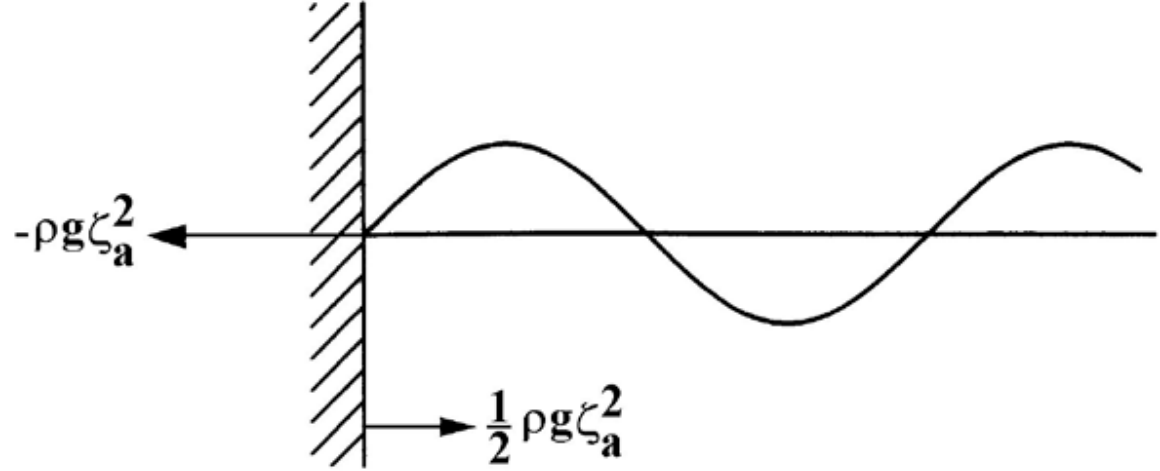
\includegraphics[width=0.3\linewidth]{figures/Theory/journee.PNG}
    \caption{Mean Wave Loads on a Wall. Source: \citep{journee2000offshore}}
    \label{fig: force on a wall journee}
\end{figure}

The second explanation for the negative forces is sought in the analogy of waves that break while approaching a simple beach. This theory is already suggested in \citet{longuethiggins1977}, where negative mean wave drift forces were observed in a submerged cylinder. In addition, \citet{Zanden2021} found negative mean wave drift forces on a submerged captive breakwater. When entering shallow water, the wave amplitude begins to increase sharply and the radiation stress increases. This must be compensated for by a decrease in hydrostatic pressure. This produces a negative tilt in the mean water surface: a wave 'set-down'. The set-down increases almost till the breaking point, after which the waves begin to lose height and the radiation stress diminishes \citep{longuethiggins1964}. The static pressure must now increase, which results in a positive tilt in the mean water level: a 'set-up'. \\
\\

\begin{figure}
    \centering
    \scalebox{0.7}{
    \begin{subfigure}[b]{0.49\textwidth}
        \centering
        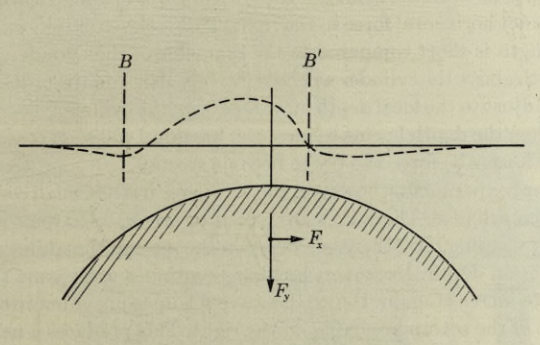
\includegraphics[width=\textwidth]{figures/Theory/longuet1.PNG}
        \caption[]%
        {{\small Wavelength short compared to the diametre of the cylinder}}    
        \label{fig: submerged cylinder longuet short}
    \end{subfigure}
    \hfill
    \begin{subfigure}[b]{0.49\textwidth}  
        \centering 
        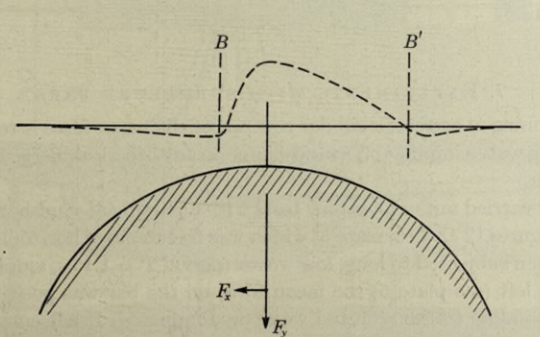
\includegraphics[width=\textwidth]{figures/Theory/longuet2.PNG}
        \caption[]%
        {{\small Wavelength short compared to the diametre of the cylinder}}    
        \label{fig: submerged cylinder lunguet long}
    \end{subfigure}
    }
    
    \caption{Schematic picture of the changes in mean level of waves in the presence of submerged cylinder. Source: \citep{longuethiggins1977}}
    \label{fig: submerged cylinders longuet}
\end{figure}

In the experiment of \citet{longuethiggins1977}, waves were breaking over a submerged cylinder, as in Figure \ref{fig: submerged cylinders longuet}. The waves were coming from the left, and the points where they started and ended their breaking are shown by B and B', respectively. If the length of the wave was short compared to the diameter of the cylinder, the mean water level was as in Figure \ref{fig: submerged cylinder longuet short}, with the set-up on the left side of the middle of the cylinder. This leads to a net horizontal force to the right. When the wave length was long compared to the diameter of the cylinder, a mean water level was found as shown in Figure \ref{fig: submerged cylinder lunguet long}. This produced a net force to the left, as shown. \\
\\
Whether the latter theory, by \citet{longuethiggins1977}, is the reason negative mean wave drift forces were found in many simulations of this thesis, is investigated by plotting the average water level of the complete simulation (minus the run-up of course). In Figure \ref{fig: average wl two configs} it can be seen that for two breakwaters that experienced a negative mean wave drift force, a set-down in front of the structure and a set-up behind the structure is present. The difference in static pressure leads to a net force to the left, against the direction of wave propagation.\\
\\




\begin{figure}[h]
    \centering
    \begin{subfigure}[b]{0.49\textwidth}
        \centering
        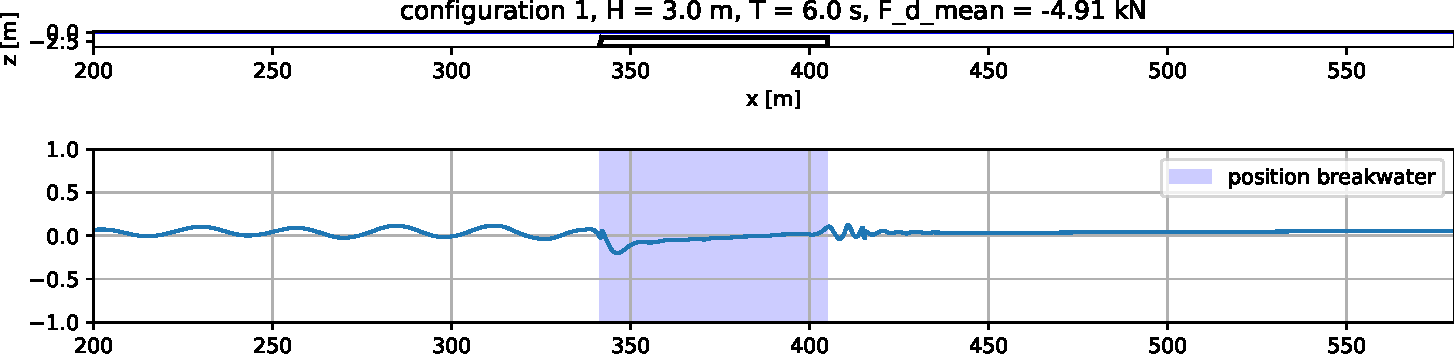
\includegraphics[width=\textwidth]{figures/ComFLOW/Results average wl/configuration1_DI1_WC1_Fd.pdf}
        \caption[]%
        {{\small }}    
        \label{}
    \end{subfigure}
    \hfill
    \begin{subfigure}[b]{0.49\textwidth}   
        \centering 
        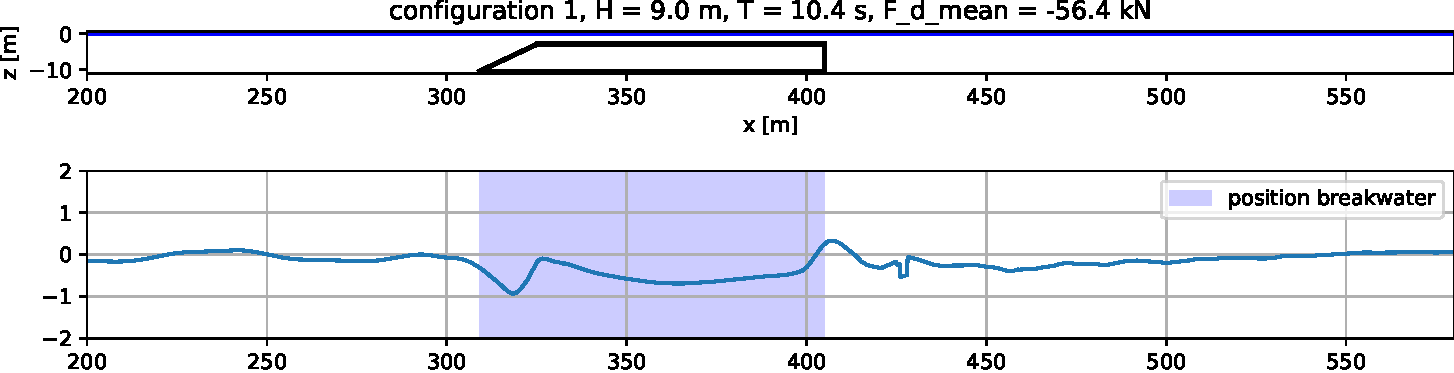
\includegraphics[width=\textwidth]{figures/ComFLOW/Results average wl/configuration1_DI1_WC2_Fd.pdf}
        \caption[]%
        {{\small }}    
        \label{}
    \end{subfigure}


    \caption{Average water level}
    \label{fig: average wl two configs}
\end{figure}


To maximise this effect and obtain the largest force to the left, the set-up must not be above the sloping beach (as in Figure \ref{fig: submerged cylinders longuet}). This might be the reason why the optimal value for the parameter "top\_fraction" did not converge to zero (which represents the largest sloping beach). This can be observed in the response surface of Figure \ref{fig: response surface top fraction}, the minimal value for top\_fraction is around 0.55 for each value of T. This effect is illustrated by comparing the breaking characteristics of configurations 18 and 69 of the design space of the second design iteration with Wave Condition 1 (see Figure \ref{fig: performance comparison sloping beach length}). The two breakwaters have a similar width W, depth T and front\_fraction, but configuration 69 has a large sloping beach (i.e. top\_fraction = 0.01) and configuration 18 has a shorter sloping beach (i.e. top\_fraction = 0.42). As can be seen in Figures \ref{fig: breaking config18} and \ref{fig: breaking config69}, the long, sloping beach causes the waves to break later. The change in depth above the structure will be relatively slow, and the height of the breaking wave will have time to adjust to the local depth of the water above the structure. This causes a set-up to be in front of the end of the sloping beach and causes, according to the theory of \citet{longuethiggins1977}, a net horizontal force force to the right on the structure. The order of magnitude of this force can be calculated as follows. The surface area of the set-up at configuration 69 (358 m <x< 405m in Figure \ref{fig:average wl config 69}) is 3.79 m$^2$, which has a weight of 3786.10 kg/m, delivers a net force of 37.14 kN/m vertically. The slope at the location of the set-up is approximately 2.2 degrees, so the horizontal contribution is  1.43 (=37.14$\cdot$tan(2.2)) kN/m, which is the order of magnitude of the difference between the two drift forces. However, the mean wave drift force on configuration 69 is still negative. Therefore, at least one other phenomenon must play a role in this negative mean wave drift force here. It might be that the low pressure region in the breaking area have a sucking effect on the structure. Or, that the fluid after breaking flows back over the sloping beach with such a high velocity that here low pressures are present and also induces a negative mean wave drift force. 

\begin{figure}[h]
    \centering
    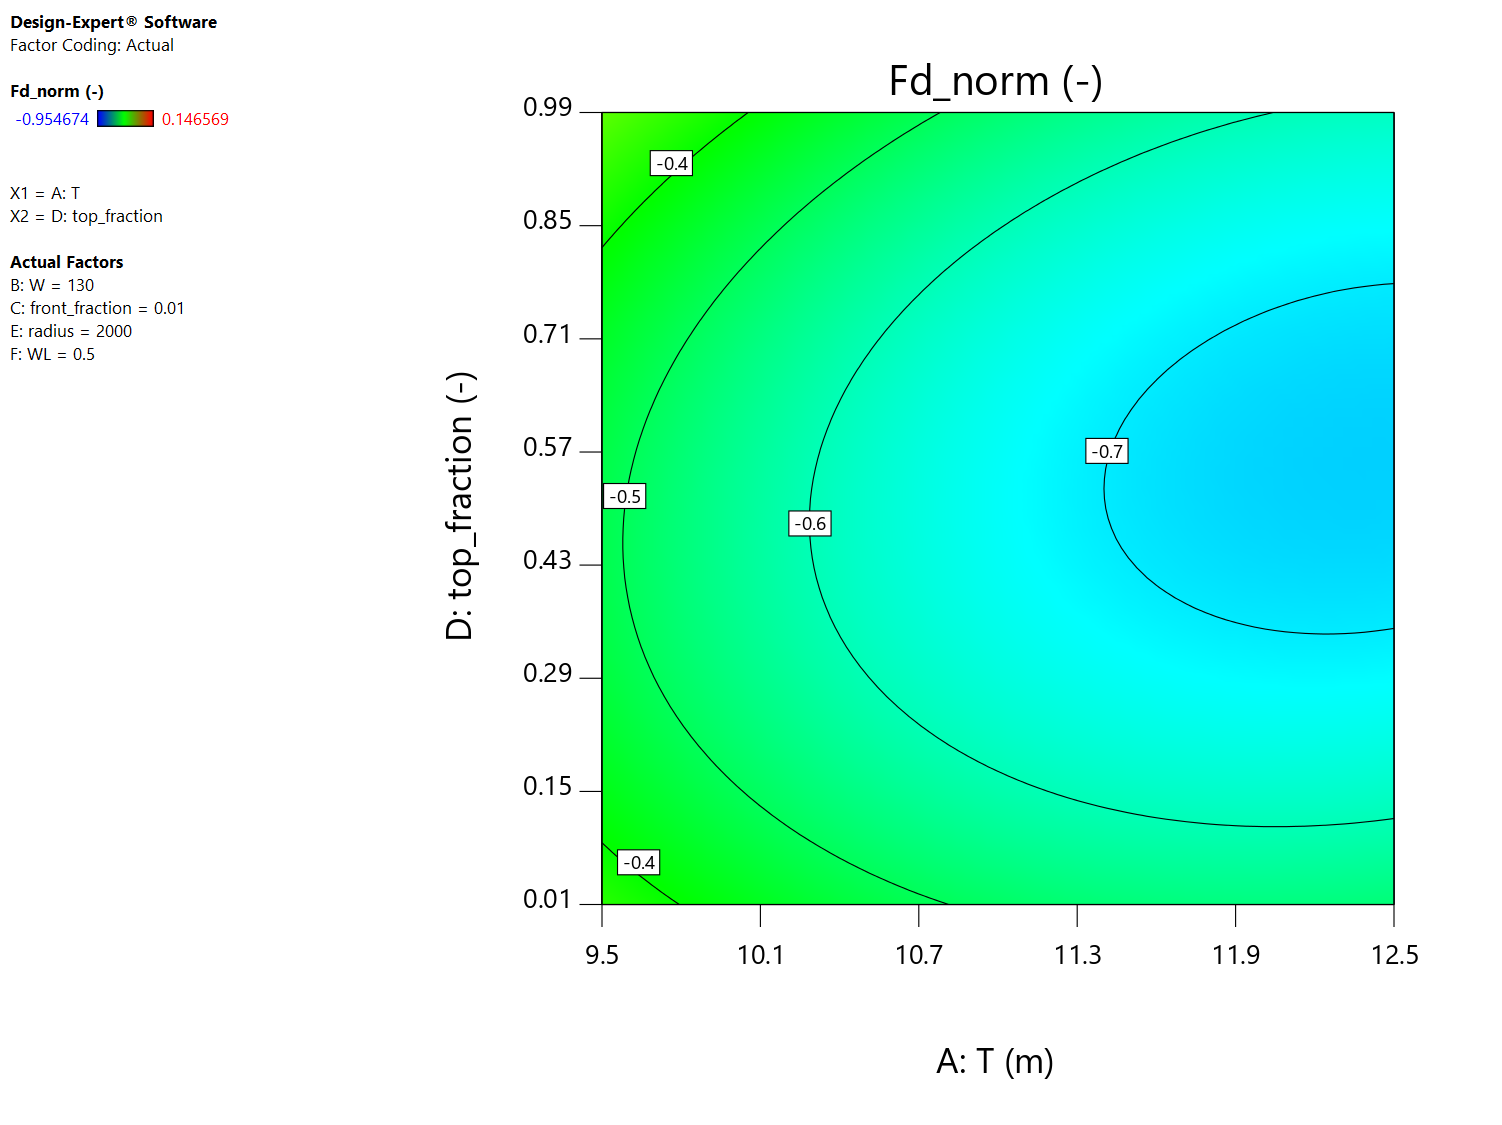
\includegraphics[width=0.49\linewidth]{figures/ComFLOW/Results DI2/Fd_front_fraction_T.png}
    \caption{Response surface, dependency of depth T and top\_fraction on mean wave drift force}
    \label{fig: response surface top fraction}
\end{figure}

\begin{figure}[h]
    \centering
    \begin{subfigure}[b]{0.49\textwidth}   
        \centering 
        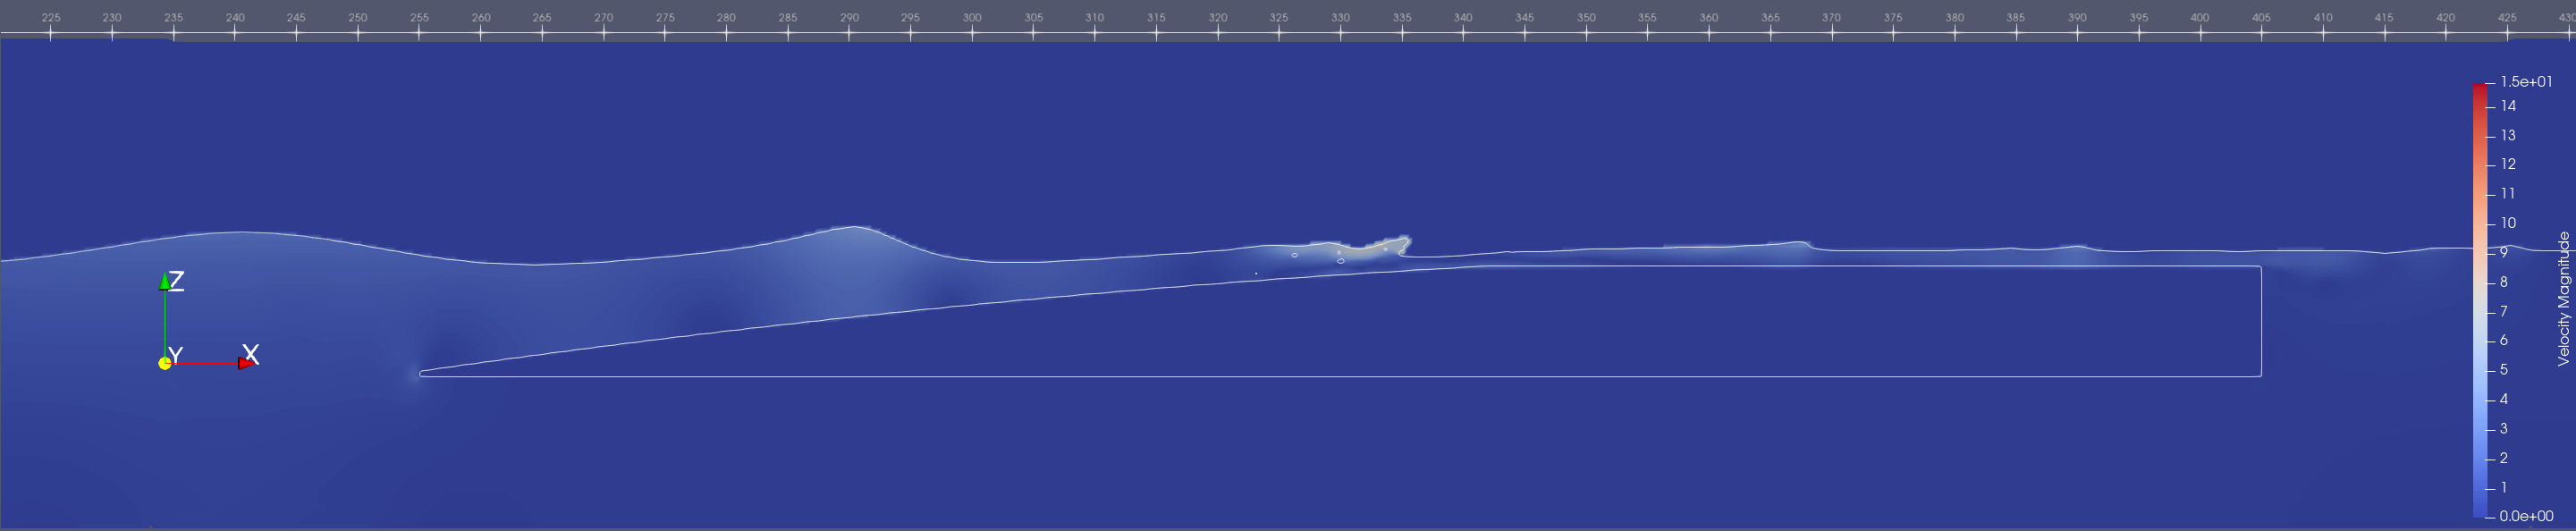
\includegraphics[width=\textwidth]{figures/ComFLOW/Results DI2/config_18_run_25_t389.png}
        \caption{Configuration 18 at t = 97.25 s}
        \label{fig: breaking config18}
    \end{subfigure}
    \hfill
    \begin{subfigure}[b]{0.49\textwidth}
        \centering
        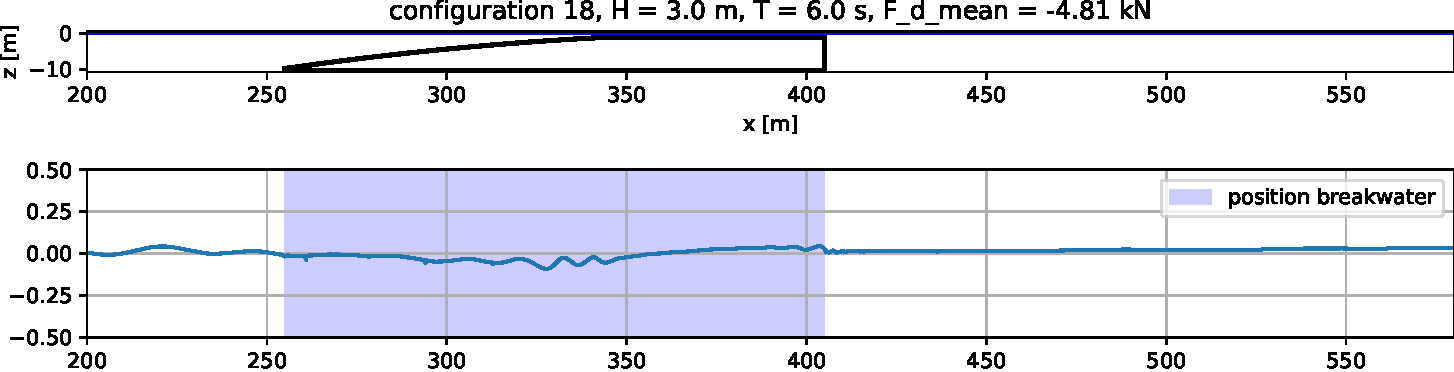
\includegraphics[width=\textwidth]{figures/ComFLOW/Results DI2/average wl/configuration18.pdf}
        \caption{Average water level configuration 18}
        \label{}
    \end{subfigure}
    \vskip\baselineskip
    \begin{subfigure}[b]{0.49\textwidth}   
        \centering 
        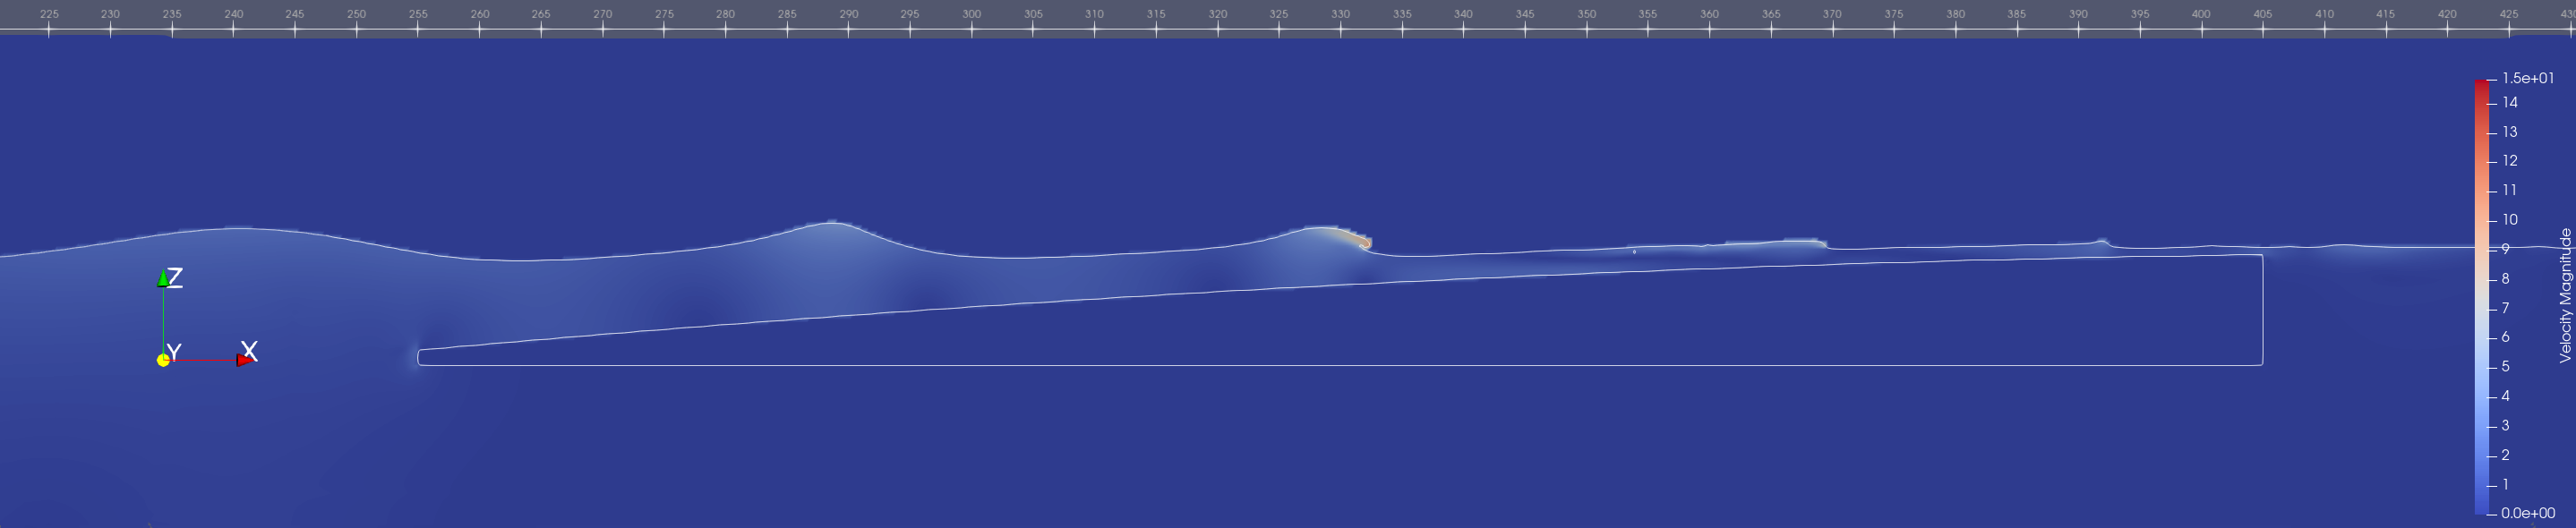
\includegraphics[width=\textwidth]{figures/ComFLOW/Results DI2/config_69_run_25_t389.png}
        \caption{Configuration 69 at t = 97.25 s}
        \label{fig: breaking config69}
    \end{subfigure}
    \hfill
    \begin{subfigure}[b]{0.49\textwidth}
        \centering
        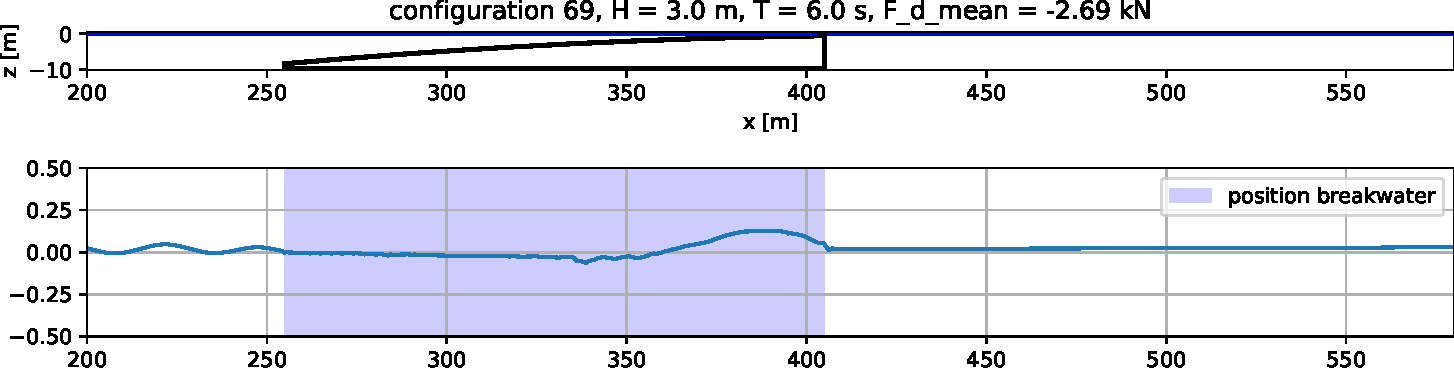
\includegraphics[width=\textwidth]{figures/ComFLOW/Results DI2/average wl/configuration69.pdf}
        \caption{Average water level configuration 69}
        \label{fig:average wl config 69}
    \end{subfigure}
    
    
    \caption{Performance comparison between short sloping beach and long sloping beach, configurations 18 and 69 of Design Iteration 2 with Wave Condition 1}
    \label{fig: performance comparison sloping beach length}   

\end{figure}




\paragraph{Maxima}
Breakwaters which experienced a high, positive mean wave drift force (in the direction of the waves) were also analysed by observing the mean water level of their simulations. They are either very reflective, which can be observed by the standing wave pattern in Figure \ref{fig: average waterlevel config91 reflective} that occurs when steep Stokes waves are reflected (\citet{maris} explained this phenomenon with figure \ref{fig: stokeswavesreflect}) . Or set-down of the mean water level occurs behind the structure for structures that cross the waterline, but the top is lower than the wave amplitude. Therefore, the waves break on top of the structure and a small stream of water flows over the breakwater and sinks to the bottom behind the structure (see Figure \ref{fig: dynamic pressure config 35}). It is not clear whether this is a physical effect or an error in the discretization of the fluid flow. If it is physical, it can be explained by a pressure difference over the water height. As waves propagate underneath the structure, the water particles behind the structure will have zero orbital velocity at the water surface and some orbital velocity around the draught of the structure. Th bis dynamic pressure difference can cause the fluid to be sucked down to the bottom. 

\begin{figure}[h]
    \centering
    \begin{subfigure}[b]{0.49\textwidth}
        \centering
        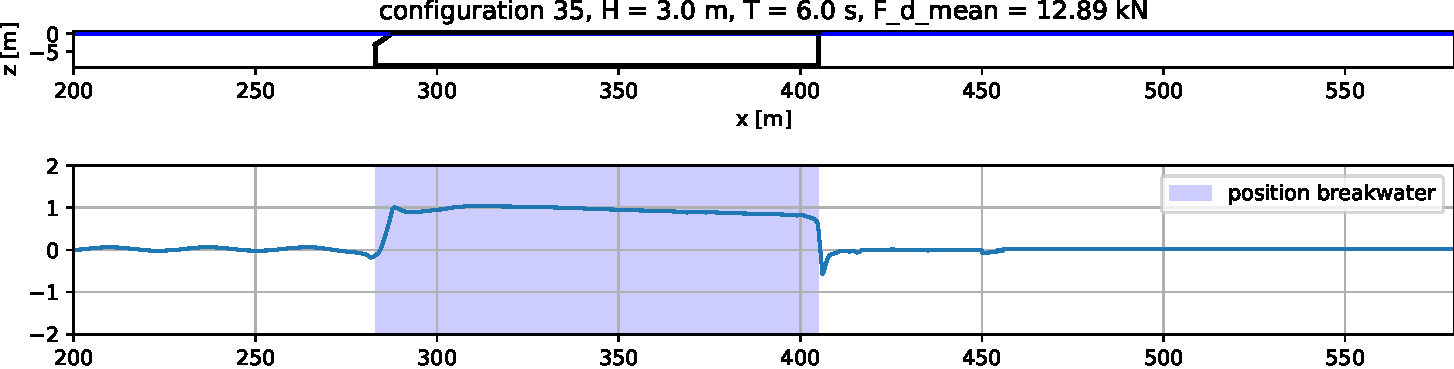
\includegraphics[width=\textwidth]{figures/ComFLOW/Results average wl/configuration35.pdf}
        \caption[]%
        {{\small }}    
        \label{fig: average waterlevel config35 setdown behind}
    \end{subfigure}
    \hfill
    \begin{subfigure}[b]{0.49\textwidth}   
        \centering 
        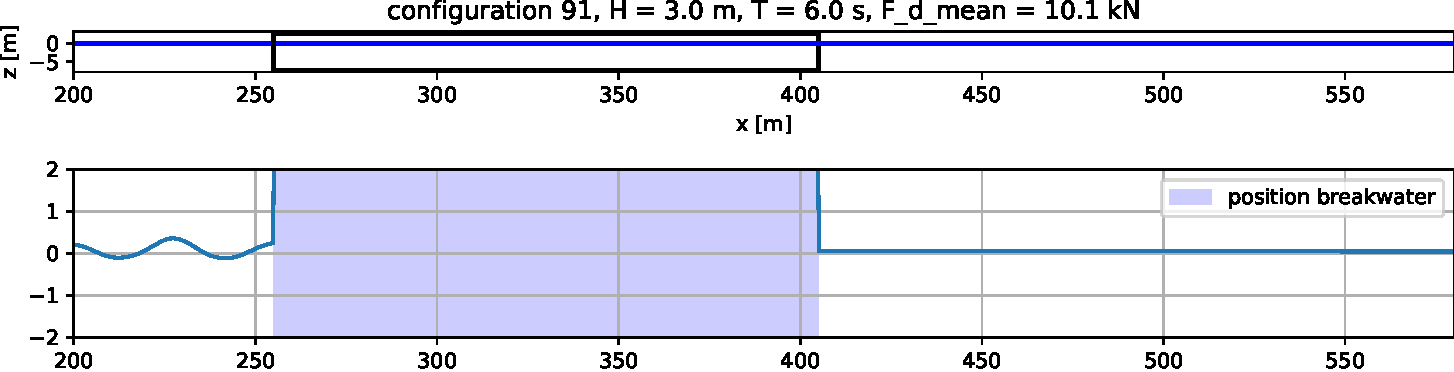
\includegraphics[width=\textwidth]{figures/ComFLOW/Results average wl/configuration91.pdf}
        \caption[]%
        {{\small }}    
        \label{fig: average waterlevel config91 reflective}
    \end{subfigure}


    \caption{Average water level for breakwaters with high mean wave drift force}
    \label{}
\end{figure}





\begin{figure}[h]
    \centering
    \begin{subfigure}[b]{0.49\textwidth}
        \centering
        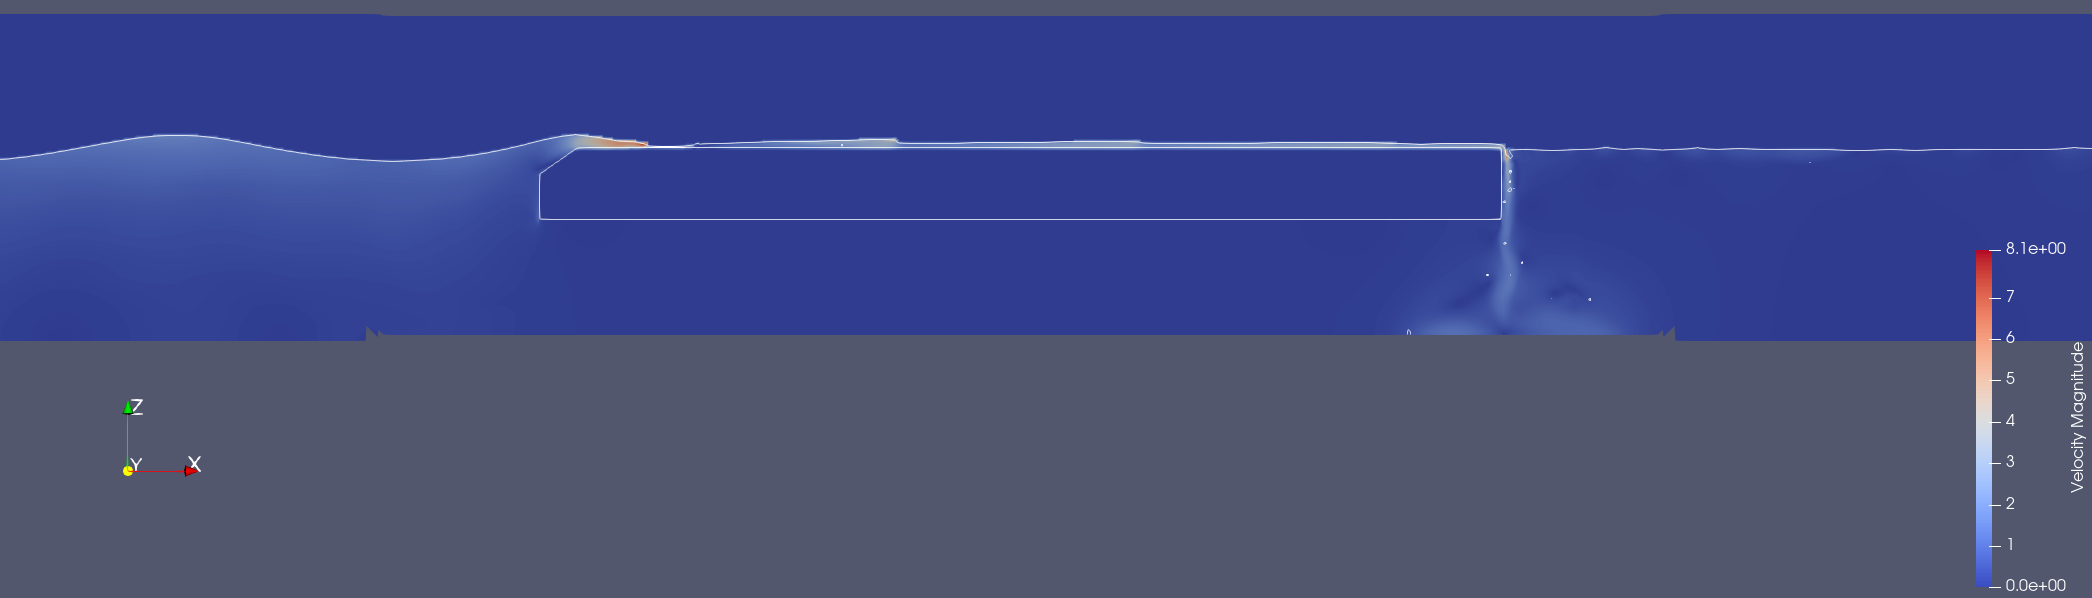
\includegraphics[width=\textwidth]{figures/ComFLOW/Results average wl/screenshot_config_35.png}
        \caption[]%
        {{\small Dynamic pressure configuration 35}}    
    \label{fig: dynamic pressure config 35}
    \end{subfigure}
    \hfill
    \begin{subfigure}[b]{0.49\textwidth}   
        \centering 
        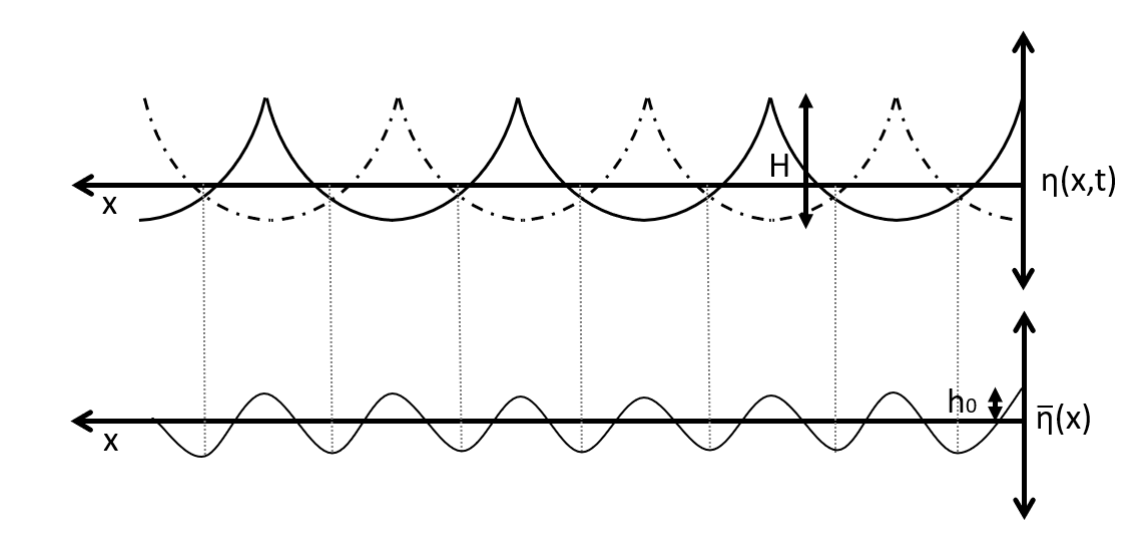
\includegraphics[width=\textwidth]{figures/Theory/standingwavepatternstokeswave.PNG}
        \caption[]%
        {{\scriptsize Top figure present the surface elevation
over the x-axis. The solid line indicates the moment t = t$_1$, in which a wave crest is present at the wall. The dash-dot line (left) presents
the moment t = t$_1$+ 1/2 T with a wave through at the wall. The bottom figure present the mean elevation of the water surface, averaged
with respect to time. Source: \citep{maris} }}    
        \label{fig: stokeswavesreflect}
    \end{subfigure}


    \caption{}
    \label{}
\end{figure}




% -effect of moving breakwaters bespreken (when pressure difference, breakwater will move in stead of experiencing that pressure difference for a long time)







\subsection{Wave transmission}
\label{sec: hydro analysis wave transmission}

Breakwaters that best attenuated the wave energy were large structures, with a high width W and depth T, which is expected according to the Macagno formula (formula \ref{eq: macagno1953}), derived from \citet{macagno1953fluid}. The design optima found to minimise the transmission coefficient often had a large sloping beach. Therefore, the characteristic of the breakwater that seems to be good at minimising the mean wave drift force (a sloping beach) is not correlated with the performance in wave attenuation.\\
\\
In Figure \ref{fig: Kt versus floater width for both wave conditions} the wave transmission coefficient K$_t$ (=H$_t$/H$_i$) is plotted against the width for all breakwaters of the design space for both wave conditions. The lines denote the Macagno relation, derived by \citet{macagno1953fluid}. This relation is derived from  linear wave theory for a box-type breakwater with infinite depth. The dependency of the draught on this formula is shown by the different lines. 

Figure \ref{fig: Kt vs W wave condition 2} shows that for Wave Condition 2, the breakwaters followed the same trend as the Macagno formula, with a constant offset lower than linear wave theory \footnote{This lower offset for the wave transmission coefficient was also observed in the validation phase of this thesis (see Figure \ref{fig:offset macagno})}.


For Wave Condition 1 (figure \ref{fig: Kt vs W wave condition 1} ) this trend is less visible (i.e. the data is more scattered). The colour of the of the dots denote the position of the breakwater with respect of the waterline, from which can be seen that the breakwaters in the top-right corner of the plot are deeply submerged. Most of the wave energy is travelling over these breakwaters, so more deviation from the Macagno formula is logical.

\begin{figure}[h]
    \centering
    \begin{subfigure}[b]{0.49\textwidth}
        \centering
        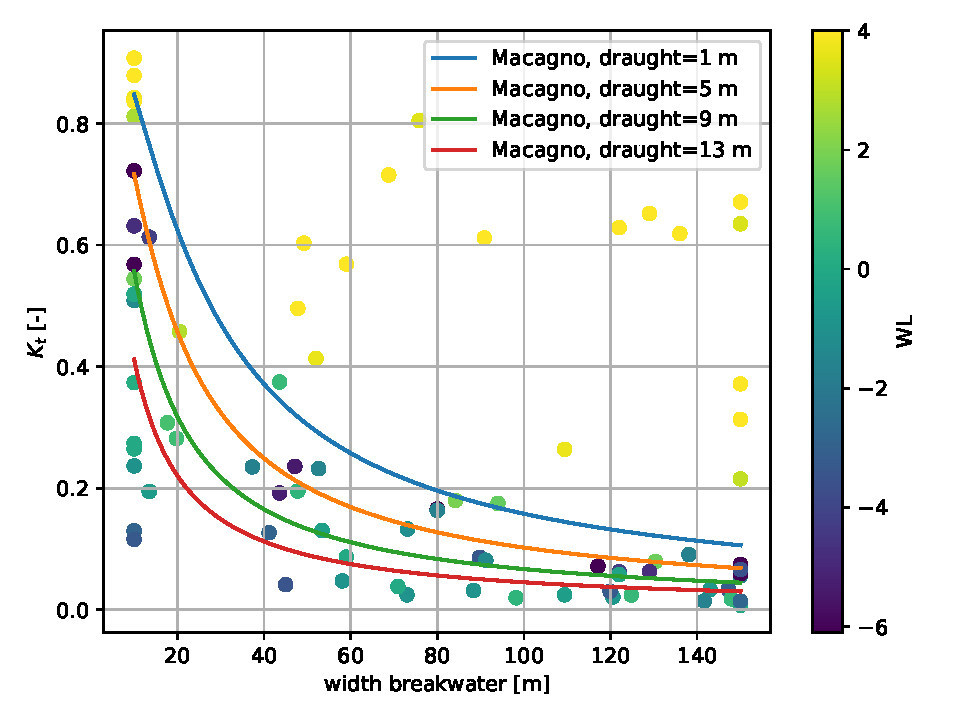
\includegraphics[width=\textwidth]{figures/ComFLOW/Results DI1/Kt_VS_W.pdf}
        \caption[]%
        {{\small Wave Condition 1: H = 3 m and T = 6.0 s}}    
        \label{fig: Kt vs W wave condition 1}
    \end{subfigure}
    \hfill
    \begin{subfigure}[b]{0.49\textwidth}  
        \centering 
        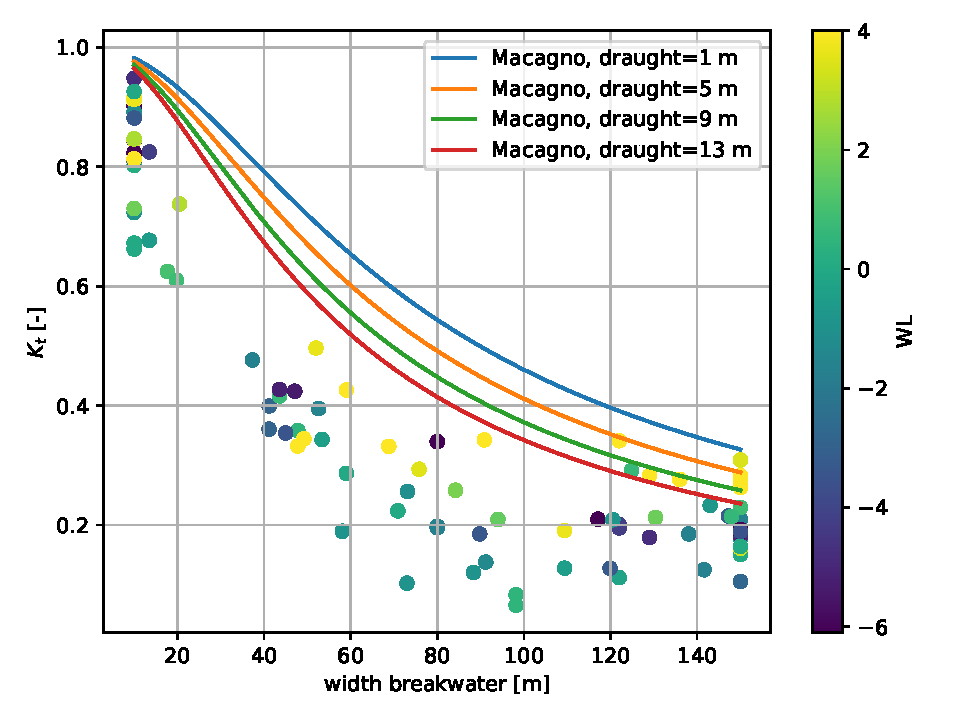
\includegraphics[width=\textwidth]{figures/ComFLOW/Results DI1 WC2 captive/Kt_VS_W.pdf}
        \caption[]%
        {{\small Wave Condition 2: H = 9 m and T = 10.4 s}}    
        \label{fig: Kt vs W wave condition 2}
    \end{subfigure}
  
    \caption{Wave transmission coefficient for breakwaters width W}
    \label{fig: Kt versus floater width for both wave conditions}
\end{figure}


% -effect of moving breakwaters bespreken; diffracted wave will be added to the transmitted wave, which will cause an irregular wave and may have larger amplitudes irregularly. On the other hand, the motion of the breakwater will cause wave energy to diffract in other directions as well, away from the island (y direction). 


